

% \begin{table*}[t]
% \centering
% \caption{Retrieval performance across different retrievalers in \textit{personabench}.}
% \label{tab:main_results}
% \resizebox{158mm}{!}{
% \begin{tabular}{lcccccccccccccc}
% \toprule
%  & \multicolumn{2}{c}{\textbf{Base}} & \multicolumn{2}{c}{\textbf{HyDE}} & \multicolumn{2}{c}{\textbf{Query2Term}} & \multicolumn{2}{c}{\textbf{MILL}} & \multicolumn{2}{c}{\textbf{CoT}} & \multicolumn{2}{c}{\textbf{ThinkQE}} & \multicolumn{2}{c}{\textbf{PBR (Ours)}} \\
% \cmidrule(r){2-3} \cmidrule(r){4-5} \cmidrule(r){6-7} \cmidrule(r){8-9} \cmidrule(r){10-11} \cmidrule(r){12-13} \cmidrule(r){14-15}
% Metrics & R@5 & N@5 & R@5 & N@5 & R@5 & N@5 & R@5 & N@5 & R@5 & N@5 & R@5 & N@5 & R@5 & N@5 \\
% \midrule
% \rowcolor{gray!15}
% \multicolumn{15}{c}{\textit{multi-qa-MiniLM-L6-cos-v1}} \\
% \textbf{Overall} & 0.4484 & 0.3669 & 0.3464 & 0.2945 & 0.3584 & 0.3060 & 0.3200 & 0.3254 & 0.3627 & 0.3000 &0.4791&0.3902& \textbf{0.5035} & \textbf{0.4201} \\
% Basic information & 0.4515 & 0.3088 & 0.3106 & 0.2395 & 0.3424 & 0.2614 & 0.2879 & 0.2337 & 0.3424 & 0.2454 &0.4606&0.3265& \textbf{0.5091} & \textbf{0.3647} \\
% Preference (hard) & 0.3659 & 0.3759 & 0.3122 & 0.3079 & 0.3659 & 0.3491 & 0.2927 & 0.4250 & 0.3171 & 0.3335 &\textbf{0.4195}&\textbf{0.4310}& 0.4049 & 0.4175 \\
% Social & 0.4852 & 0.4356 & 0.3909 & 0.3259 & 0.3494 & 0.3144 & 0.3808 & 0.3923 & 0.4009 & 0.3320 &0.5503&0.4554& \textbf{0.5541} & \textbf{0.4914} \\
% Preference (easy) & 0.4904 & 0.4582 & 0.4615 & 0.4422 & 0.4327 & 0.4095 & 0.3750 & 0.4195 & 0.4423 & 0.4133 &0.5064&0.4626& \textbf{0.5321} & \textbf{0.5129} \\
% \midrule
% \rowcolor{gray!15}
% \multicolumn{15}{c}{\textit{all-MiniLM-L6-v2}} \\
% \textbf{Overall} & 0.3783 & 0.3074 & 0.3747 & 0.3144 & 0.3908 & 0.3256 & 0.3030 & 0.3059 & 0.3721 & 0.3098 &0.3861&0.3393& \textbf{0.4516} & \textbf{0.3855} \\
% Basic information & 0.3515 & 0.2644 & 0.4015 & 0.2975 & 0.3894 & 0.2914 & 0.3030 & 0.2547 & 0.3455 & 0.2696 &0.3455&0.2677& \textbf{0.4515} & \textbf{0.3485} \\
% Preference (hard) & 0.4000 & 0.3547 & 0.3512 & 0.3561 & 0.3805 & 0.3798 & 0.3220 & 0.4171 & 0.3463 & 0.3490 &0.3366&0.3486& \textbf{0.4341} & \textbf{0.4352} \\
% Social & 0.3921 & 0.3048 & 0.2805 & 0.2435 & 0.3984 & 0.3163 & 0.2638 & 0.2829 & 0.4160 & 0.3046 &\textbf{0.4780}&\textbf{0.4334}& 0.4494 & 0.3777 \\
% Preference (easy) & 0.4295 & 0.4199 & \textbf{0.4904} & 0.4646 & 0.3974 & 0.4038 & 0.3526 & 0.3944 & 0.4359 & 0.4285 &0.4487&0.4357& 0.4840 & \textbf{0.4800} \\
% \midrule
% \rowcolor{gray!15}
% \multicolumn{15}{c}{\textit{bge-base-en-v1.5}} \\
% \textbf{Overall} & 0.3738 & 0.3015 & 0.3108 & 0.2597 & 0.3007 & 0.2497 & 0.2791 & 0.2869 & 0.3199 & 0.2642 &0.3643&0.3156& \textbf{0.4029} & \textbf{0.3402} \\
% Basic information & 0.3970 & 0.2748 & 0.2955 & 0.2051 & 0.3000 & 0.1955 & 0.2879 & 0.2319 & 0.3152 & 0.2052 &0.3152&0.2430& \textbf{0.4121} & \textbf{0.3057} \\
% Preference (hard) & 0.3268 & 0.3343 & 0.3073 & 0.3148 & 0.2976 & 0.3186 & 0.2244 & 0.3566 & 0.3073 & 0.3281 &0.3463&0.3635& \textbf{0.3707} & \textbf{0.3889} \\
% Social & 0.3204 & 0.2799 & 0.2714 & 0.2443 & 0.2852 & 0.2503 & 0.2752 & 0.3004 & 0.2965 & 0.2647 &\textbf{0.4261}&\textbf{0.3735}& 0.3657 & 0.3089 \\
% Preference (easy) & 0.4583 & 0.4065 & 0.4615 & 0.4356 & 0.3397 & 0.3693 & 0.3365 & 0.3819 & 0.4071 & 0.4117 &0.4744&0.4289& \textbf{0.4904} & \textbf{0.4734} \\
% \midrule
% \textbf{Overall Average} & 0.4002 & 0.3253 & 0.3440 & 0.2895 & 0.3500 & 0.2938 & 0.3007 & 0.3061 & 0.3295 & 0.3121 &0.4098& 0.3484& \textbf{0.4527} & \textbf{0.3819} \\
% \bottomrule
% \end{tabular}
% }
% \vspace{-10pt}
% \end{table*}

\begin{table*}[ht]
\centering
\small
\setlength\tabcolsep{2.2pt}  %可以控制列间距
\renewcommand{\arraystretch}{0.80} %可以控制行间距
% \resizebox{160mm}{!}{
\begin{tabular}{lcccccccccccc}
\toprule
 \textbf{Dataset} & \multicolumn{6}{c}{\textbf{LongMenEval-s}} & \multicolumn{6}{c}{\textbf{LongMenEval-m}} \\
 \cmidrule(lr){2-7} \cmidrule(lr){8-13}
Metrics & R@1 & N@1 & R@3 & N@3 & R@5 & N@5 & R@1 & N@1 & R@3 & N@3 & R@5 & N@5 \\
\midrule
\rowcolor{gray!15}
\multicolumn{13}{c}{\textit{multi-qa-MiniLM-L6-cos-v1}} \\
Base     & 0.1885 & 0.7924 & 0.6730 & 0.8020 & 0.8067 & 0.8301 & 0.1098 & \underline{0.5251} & 0.4057 & 0.5559 & 0.5394 & 0.6038 \\
HyDE     & \underline{0.1957} & 0.7852 & 0.6945 & 0.8173 & 0.8115 & \underline{0.8436} & 0.1146 & 0.4964 & 0.4129 & 0.5411 & 0.5179 & 0.5828 \\
Query2Term & 0.1814 & 0.7446 & 0.6396 & 0.7684 & 0.7470 & 0.7959 & 0.1146 & 0.4749 & 0.3747 & 0.5091 & 0.4821 & 0.5531 \\
MILL     & 0.1838 & 0.7709 & 0.6635 & 0.7845 & 0.6635 & 0.7712 & 0.1122 & 0.5155 & 0.4129 & 0.5552 & 0.4129 & 0.5468 \\
CoT      & 0.1862 & 0.7470 & 0.6516 & 0.7707 & 0.7542 & 0.8006 & 0.1098 & 0.4654 & 0.3866 & 0.5110 & 0.4726 & 0.5475 \\
ThinkQE & 0.1933 & \underline{0.8019} & \underline{0.7064} & \underline{0.8214} & \underline{0.8162 }& 0.8424 & \underline{0.1169} & 0.5227 & \underline{0.4168} & \underline{0.5647} & \underline{0.5517} & \underline{0.6156} \\
\textbf{PBR} & $\mathbf{0.2100^*}$ & $\mathbf{0.8210^*}$ & $\mathbf{0.7279^*}$ & $\mathbf{0.8444^*}$ & $\mathbf{0.8282^*}$ & $\mathbf{0.8598^*}$ & $\mathbf{0.1217^*}$ & $\mathbf{0.5537^*}$ & $\mathbf{0.4320^*}$ & $\mathbf{0.5776^*}$ & $\mathbf{0.5537^*}$ & $\mathbf{0.6177^*}$ \\
\midrule
\rowcolor{gray!15}
\multicolumn{13}{c}{\textit{all-MiniLM-L6-v2}}\\
Base     & \underline{0.2196} & \underline{0.8234} & \underline{0.7399} & \underline{0.8477} & \underline{0.8568} & \underline{0.8731} & \underline{0.1265} & 0.5322 & 0.4415 & 0.5857 & 0.5346 & 0.6191 \\
HyDE     & 0.2172 & 0.8138 & 0.7208 & 0.8372 & 0.8377 & 0.8599 & 0.1074 & 0.4988 & 0.4081 & 0.5483 & 0.5131 & 0.5884 \\
Query2Term & \underline{0.2196} & 0.8019 & 0.6778 & 0.8000 & 0.8138 & 0.8351 & 0.1193 & 0.4940 & 0.3747 & 0.5209 & 0.4964 & 0.5689 \\
MILL     & 0.2100 & 0.8162 & 0.7208 & 0.8382 & 0.7208 & 0.8257 & 0.1217 & 0.5179 & 0.3962 & 0.5530 & 0.3962 & 0.5450 \\
CoT      & 0.2124 & 0.7709 & 0.6730 & 0.7932 & 0.7780 & 0.8187 & 0.1193 & 0.4487 & 0.3389 & 0.4920 & 0.4344 & 0.5273 \\
ThinkQE & \underline{0.2196} & \underline{0.8234} & 0.7232 & 0.8332 & 0.8162 & 0.8527 & 0.1241 & \underline{0.5585} & \underline{0.4461} & \underline{0.5871} & \underline{0.5537} & \underline{0.6229} \\
\textbf{PBR} & $\mathbf{0.2267^*}$ & $\mathbf{0.8592^*}$ & $\mathbf{0.7780^*}$ & $\mathbf{0.8754^*}$ & $\mathbf{0.8640^*}$ & $\mathbf{0.8902^*}$ & $\mathbf{0.1408^*}$ & $\mathbf{0.5800^*}$ & $\mathbf{0.4463^*}$ & $\mathbf{0.5949^*}$ & $\mathbf{0.5847^*}$ & $\mathbf{0.6424^*}$ \\
\midrule
\rowcolor{gray!15}
\multicolumn{13}{c}{\textit{bge-base-en-v1.5}} \\
Base     & \underline{0.2267} & 0.8616 & 0.7900 & 0.8863 & 0.8926 & 0.9007 & 0.1217 & 0.5943 & \underline{0.5322} & \underline{0.6605} & 0.6444 & 0.6929 \\
HyDE     & 0.2196 & 0.8759 & 0.7995 & 0.8974 & 0.8998 & 0.9044 & 0.1313 & 0.5943 & 0.5298 & 0.6538 & \underline{0.6659} & 0.7010 \\
Query2Term & 0.2100 & 0.8544 & 0.7637 & 0.8739 & 0.8926 & 0.8989 & 0.1360 & 0.5776 & 0.5155 & 0.6290 & 0.6348 & 0.6754 \\
MILL     & \underline{0.2267} & 0.8663 & 0.7804 & 0.8819 & 0.7804 & 0.8680 & 0.1289 & 0.5967 & 0.5107 & 0.6362 & 0.5107 & 0.6278 \\
CoT      & 0.2196 & 0.8425 & 0.7637 & 0.8707 & 0.8783 & 0.8918 & \underline{0.1384} & 0.5609 & 0.4964 & 0.6148 & 0.5967 & 0.6570 \\
ThinkQE & 0.2124 & \underline{0.8807} & \underline{0.8108} & \underline{0.9012} & \underline{0.9021} & \underline{0.9126} & 0.1384 & \underline{0.6072} & 0.5080 & 0.6321 & 0.6445 & \underline{0.7013} \\
\textbf{PBR} & $\mathbf{0.2315^*}$ & $\mathbf{0.8902^*}$ & $\mathbf{0.8138^*}$ & $\mathbf{0.9072^*}$ & $\mathbf{0.9045^*}$ & $\mathbf{0.9191^*}$ & $\mathbf{0.1408^*}$ & $\mathbf{0.6205^*}$ & $\mathbf{0.5489^*}$ & $\mathbf{0.6612^*}$ & $\mathbf{0.6874^*}$ & $\mathbf{0.7060^*}$\\
\bottomrule
\end{tabular}
% }
\caption{Retrieval performance in \textbf{LongMemEval}. The best results are in \textbf{bold}, and the second-best results are \underline{underlined}. ``\textbf{{\Large *}}'' indicates the statistically significant improvements (i.e., two-sided t-test with $p<0.05$) over the best baseline. }
\label{tab:longmen_results}
\vspace{-10pt}
\end{table*}



\section{Experiment}


In this section, we conduct experiments to address the following research questions:
% We address the following research questions:
\begin{itemize}[leftmargin=*]
    \item \textbf{RQ1}: \emph{Does the proposed PBR method improve retrieval performance on personalized corpus?}
    \item \textbf{RQ2}: \emph{What are the individual contributions of the P-PRF and P-Anchor modules to the overall performance?}
    % \item \textbf{RQ3}: \emph{Can P-PRF improve model performance by generating pseudo signals that enhance both the widely (semantic diversity) and deeply (reasoning granularity)?}
    \item \textbf{RQ3}: \emph{How does information propagation within the P-Anchor module affect the alignment between the query and user-specific corpora?}
\end{itemize}

\subsection{Experiment Setting}

\paragraph{Datasets.}
We evaluate our method on two recent benchmarks tailored for personalized retrieval. \textbf{PersonaBench}~\cite{tan2025personabench} simulates user-specific queries over synthetic private data (e.g., preferences, behaviors, demographics), requiring models to align responses with personalized context. It includes both explicit and implicit user traits across diverse domains. \textbf{LongMemEval}~\cite{wu2025longmemeval} targets long-term interactive memory, where each user is associated with multi-turn dialogue traces. We use two subsets: \textit{LongMemEval-s} (sparse history) and \textit{LongMemEval-m} (dense history), to evaluate the effectiveness of retrieval under both short- and long-horizon personalization. More details are provided in Appendix 1.

\paragraph{Evaluation Metrics.}
We report performance using two standard retrieval metrics: \textbf{Recall@K (R@K)}, which measures the proportion of relevant items ranked within the top-K retrieved results, and \textbf{NDCG@K (N@K)} to reflect retrieval quality.
% Following common RAG practice~\cite{tan2025personabench,wu2025longmemeval}, we evaluate at $K \in \{1, 3, 5\}$ across all settings.

\paragraph{Baselines.}
% \pengyue{six}
% \pengyue{citation}
We compare our method with six strong baselines: \textbf{Base}, a static query retriever without expansion; \textbf{HyDE}~\cite{gao2023precise}, which generates hypothetical answers to guide retrieval; \textbf{Query2Term}~\cite{jagerman2023query}, which performs keyphrase-based query expansion; \textbf{MILL}~\cite{jia2023mill}, which leverages multi-level logical structures; \textbf{CoT}~\cite{wei2022chain}, which applies chain-of-thought reasoning for better ranking; and \textbf{ThinkQE}~\cite{lei2025thinkqe}. 

\paragraph{Implement details.}
% To verify the robustness of our approach, all methods are evaluated under three retrieval backbones: \texttt{multi-qa-MiniLM-L6-cos-v1}\footnote{https://huggingface.co/sentence-transformers/multi-qa-MiniLM-L6-cos-v1}, \texttt{all-MiniLM-L6-v2}\footnote{https://huggingface.co/sentence-transformers/all-MiniLM-L6-v2}, and \texttt{bge-base-en-v1.5}\footnote{https://huggingface.co/BAAI/bge-base-en-v1.5}. For a fair comparison, all query expansions are generated using GPT-4o-mini~\cite{achiam2023gpt}. In our \textbf{PBR} framework, we set $k_1=5$,$m=5$, $\theta=0.75$, and $k_2=10$ across \textit{Perosnabench} and \textit{LongMemEval-s}. The larger $k_2=50$ is particularly suited for \textit{LongMemEval-m}, which contains richer user histories. More details are provided in Appendix 2.
% To verify the robustness of PBR, all methods are evaluated under three retrieval backbones: \texttt{multi-qa-MiniLM-L6-cos-v1}~\cite{wang2020minilm}, \texttt{all-MiniLM-L6-v2}~\cite{wang2020minilm}, and \texttt{bge-base-en-v1.5}~\cite{chen2024bge}. For a fair comparison, all methods are using GPT-4o-mini~\cite{achiam2023gpt}, and run 5 times. In \textbf{PBR} framework, we set $k_1=5$,$m=5$, $\theta=0.75$, and $k_2=10$ across \textit{Perosnabench} and \textit{LongMemEval-s}. The larger $k_2=50$ is particularly suited for \textit{LongMemEval-m}, which contains richer user histories. More details are provided in Appendix 2.
To verify the robustness of PBR, all methods are evaluated under three retrieval backbones: \texttt{multi-qa-MiniLM-L6-cos-v1}~\cite{wang2020minilm}, \texttt{all-MiniLM-L6-v2}~\cite{wang2020minilm}, and \texttt{bge-base-en-v1.5}~\cite{chen2024bge}. For a fair comparison, all methods use an advanced LLM and run 5 times. In \textbf{PBR} framework, we set $k_1=5$,$m=5$, $\theta=0.75$, and $k_2=10$ across \textit{Perosnabench} and \textit{LongMemEval-s}. The larger $k_2=50$ is particularly suited for \textit{LongMemEval-m}, which contains richer user histories. More details are provided in Appendix 2.


\subsection{Overall Performance (RQ1)}


\begin{figure*}[ht]
    \centering
    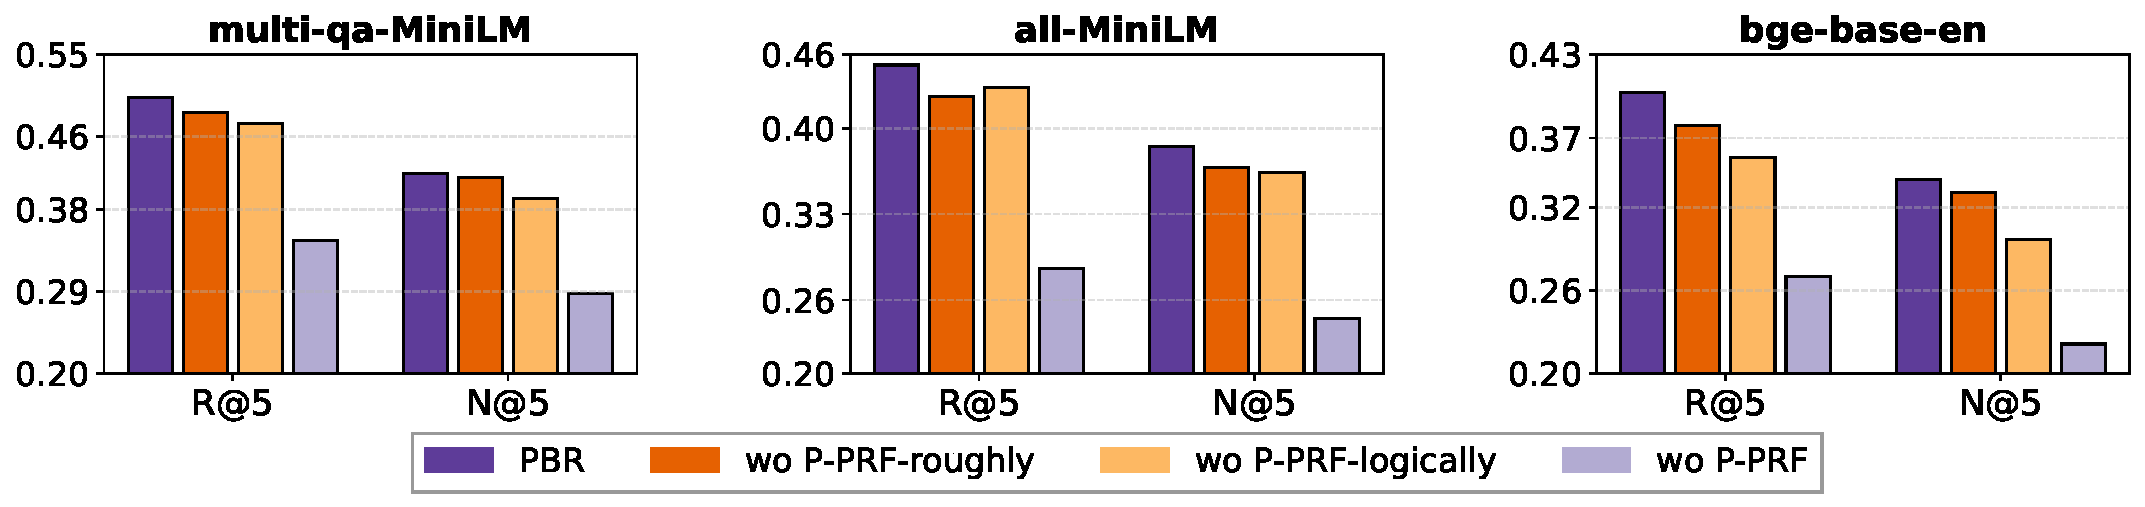
\includegraphics[width=0.9\linewidth]{figure/3x1_dataset_comparison.pdf}
    \caption{%
        Overall performance in \textbf{PersonaBench} comparison across three retrieval models. 
    }
    \label{fig:pprf-ablation}
    \vspace{-10pt}
\end{figure*}

\begin{figure*}[ht]
    \centering
    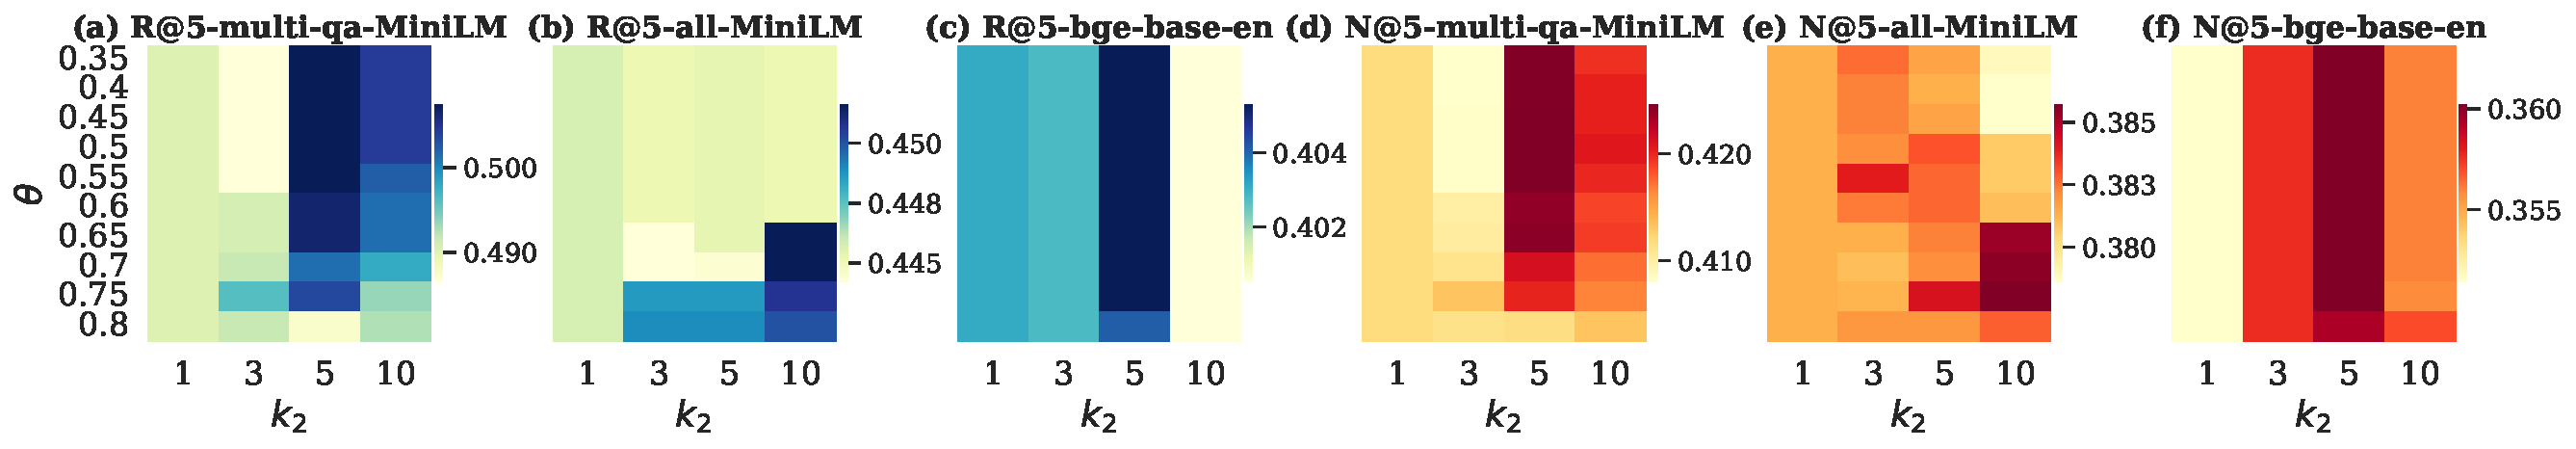
\includegraphics[width=1.0\linewidth]{figure/heatmaps_1x6.pdf}
    \caption{Parameter sensitivity analysis on P-Anchor of $\theta$ and $k_2$ settings.}
     % \pengyue{fontsize is too small}
    \label{fig:anchor_sensitivity}
    \vspace{-10pt}
\end{figure*}



To comprehensively evaluate the effectiveness of PBR, we conduct experiments on two benchmarks. \textbf{PersonaBench} contains 6 users, each with a dedicated corpus and about 50 user queries characterized by ambiguous intent and highly personalized language. In contrast, \textbf{LongMemEval} simulates a large-scale factual QA scenario with 500 distinct user queries, each paired with a relevant memory corpus. The former highlights soft personalization challenges (e.g., preferences and social traits), while the latter emphasizes hard factual grounding under long-context retrieval.

\textbf{PBR resolving semantic ambiguity through user-specific expansion.} 
Queries in PersonaBench often exhibit semantic openness and personal references—such as ``Where is my hometown?'' or ``What is my favorite color?''—which cannot be resolved without grounding in the user's unique corpus. As shown in Table~\ref{tab:main_results}, our PBR framework achieves the best overall performance across all retrievers (R@5: \textbf{0.4527}, N@5: \textbf{0.3819}), significantly surpassing the best baseline (ThinkQE: \underline{0.4098} / \underline{0.3484}). This gain stems from PBR’s ability to generate user-style pseudo-feedback that anchors the query into a meaningful semantic space, reducing ambiguity and improving retrieval accuracy. 

\textbf{PBR excels in factual retrieval by boosting top-ranked precision.} 
In contrast to PersonaBench, queries in LongMemEval are fact-oriented with specific personalization requirements, each associated with a specific memory corpus. In this setting, PBR boosts top-ranked retrieval performance. In Table~\ref{tab:longmen_results}, PBR also outperforms all baselines on LongMemEval, particularly on R@1, where it achieves \textbf{0.2315} on the -s version and \textbf{0.1408} on the -m version using \texttt{bge}. Compared to the best-performing baseline (0.2267 / 0.1384), PBR achieves absolute gain on top-1 precision. This suggests that our style simulation and structural anchoring more precisely locate relevant memory, elevating correct answers to top-1 even in long-context settings.

\subsection{Ablation Study (RQ2)}
To investigate the individual roles of \textbf{P-PRF} and \textbf{P-Anchor} in our framework, we perform a module-wise ablation across three retrievers in PersonaBench, as shown in Table~\ref{tab:ablation_results}. Each model variant is evaluated under both R@5 and N@5. More details are provided in Appendix 3.

\begin{table}[ht]
\centering
\renewcommand{\arraystretch}{0.90} %可以控制行间距
\resizebox{85mm}{!}{
\begin{tabular}{lcccccc}
\toprule
& \multicolumn{2}{c}{\textbf{PBR}} 
& \multicolumn{2}{c}{\textbf{w/o P-Anchor}} 
& \multicolumn{2}{c}{\textbf{w/o P-PRF}}\\
\cmidrule(lr){2-3} \cmidrule(lr){4-5} \cmidrule(lr){6-7} 
Metrics & R@5 & N@5 & R@5 & N@5 & R@5 & N@5   \\
\midrule
\rowcolor{gray!15}
\multicolumn{7}{c}{\textit{multi-qa-MiniLM-L6-cos-v1}} \\
Overall & \textbf{0.5035} & \textbf{0.4201} & 0.4871 & 0.4100 & 0.3457 & 0.2877 \\
Basic information & \textbf{0.5091} & \textbf{0.3647} & 0.4833 & 0.3570 & 0.3318 & 0.2242 \\
Preference (hard) & 0.4049 & 0.4175 & \textbf{0.4390} & \textbf{0.4295} & 0.2683 & 0.2981  \\
Social & \textbf{0.5541} & \textbf{0.4914} & 0.5164 & 0.4529 & 0.4277 & 0.3851 \\
Preference (easy) & \textbf{0.5321} & \textbf{0.5129} & 0.5192 & 0.5160 & 0.3590 & 0.3414 \\
\midrule
\rowcolor{gray!15}
\multicolumn{7}{c}{\textit{all-MiniLM-L6-v2}}\\
Overall & \textbf{0.4516} & \textbf{0.3855} & 0.4382 & 0.3729 & 0.2860 & 0.2449 \\
Basic information & \textbf{0.4515} & \textbf{0.3485} & 0.4379 & 0.3393 & 0.1985 & 0.1617 \\
Preference (hard) & \textbf{0.4341} & \textbf{0.4352} & 0.4244 & 0.4201 & 0.2878 & 0.2718 \\
Social & \textbf{0.4494} & \textbf{0.3777} & 0.4333 & 0.3639 & 0.4179 & 0.3387 \\
Preference (easy) & \textbf{0.4840} & \textbf{0.4800} & 0.4712 & 0.4587 & 0.3846 & 0.3634  \\
\midrule
\rowcolor{gray!15}
\multicolumn{7}{c}{\textit{BAAI/bge-base-en-v1.5}} \\ 
Overall & \textbf{0.4029} & \textbf{0.3402} & 0.3921 & 0.3256 & 0.2699 & 0.2214  \\
Basic information & \textbf{0.4121} & \textbf{0.3057} & 0.3970 & 0.2958 & 0.2576 & 0.1804 \\
Preference (hard) & 0.3707 & \textbf{0.3889} & \textbf{0.3902} & 0.3778 & 0.2146 & 0.2173  \\
Social & \textbf{0.3657} & \textbf{0.3089} & 0.3431 & 0.2822 & 0.3261 & 0.2816  \\
Preference (easy) & \textbf{0.4904} & \textbf{0.4734} & 0.4744 & 0.4582 & 0.2949 & 0.2785  \\
\midrule
\textbf{Average} & \textbf{0.4527} & \textbf{0.3819} & 0.4391 & 0.3695 & 0.3005 & 0.2513 \\
\bottomrule
\end{tabular}
}
\caption{Ablation study of PBR in \textbf{PersonaBench}.}
\label{tab:ablation_results}
\vspace{-10pt}
\end{table}



\textbf{P-PRF drives major performance gains in personalized retrieval.}
Removing P-PRF leads to a substantial performance drop across all retrievers (e.g., on all-MiniLM, R@5 falls from 0.4516 to 0.2860), with the most severe decline observed on personalization-heavy subsets. This underscores the importance of P-PRF in generating semantically rich and stylistically aligned pseudo queries that effectively capture user intent.

\textbf{Effectiveness of P-PRF Components.}
To assess how \textbf{P-PRF} enhances intent modeling, we perform ablation studies in PersonaBench and three retrievers (Figure~\ref{fig:pprf-ablation}). Removing either the \textit{roughly}-aligned pseudo-utterance or \textit{logically}-structured pseudo-reasoning consistently degrades performance in R@5 and N@5. The former harms lexical coverage, while the latter impairs goal-oriented reasoning, reducing ranking precision on inference-heavy datasets.

\textbf{P-Anchor promotes semantic alignment in structured corpora.}
Removing P-Anchor leads to a consistent drop (e.g., N@5 from \textbf{0.3819} to 0.3695), especially in \textit{Basic Information} and \textit{Social}, where user corpora exhibit clearer structure. In contrast, in non-clustered tasks like \textit{Preference (hard)}, it offers limited gain and may overfit. P-Anchor is most effective when user context is semantically coherent.

\subsection{Parameter Sensitivity Analysis (RQ3)}



\begin{figure*}[ht]
  \centering
  \begin{subfigure}[t]{0.32\textwidth}
    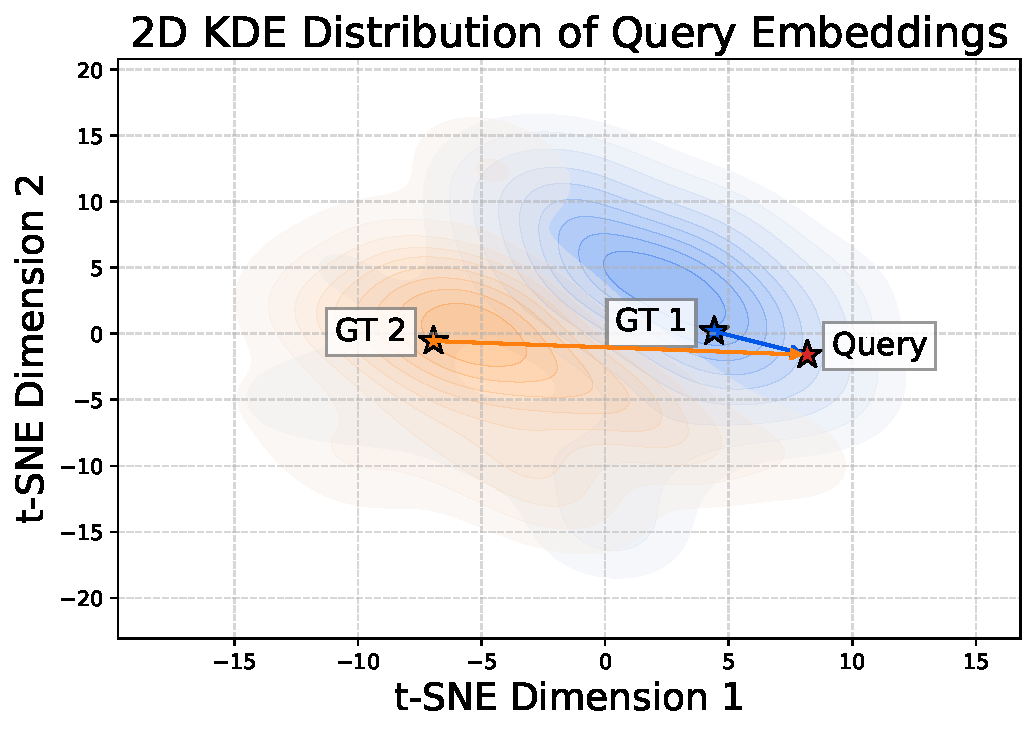
\includegraphics[width=1.0\linewidth]{figure/figure1_query_gt.pdf}
    \caption{Query-GT Comparison}
    \label{fig:query_gt}
  \end{subfigure}
  \hfill
  \begin{subfigure}[t]{0.32\textwidth}
    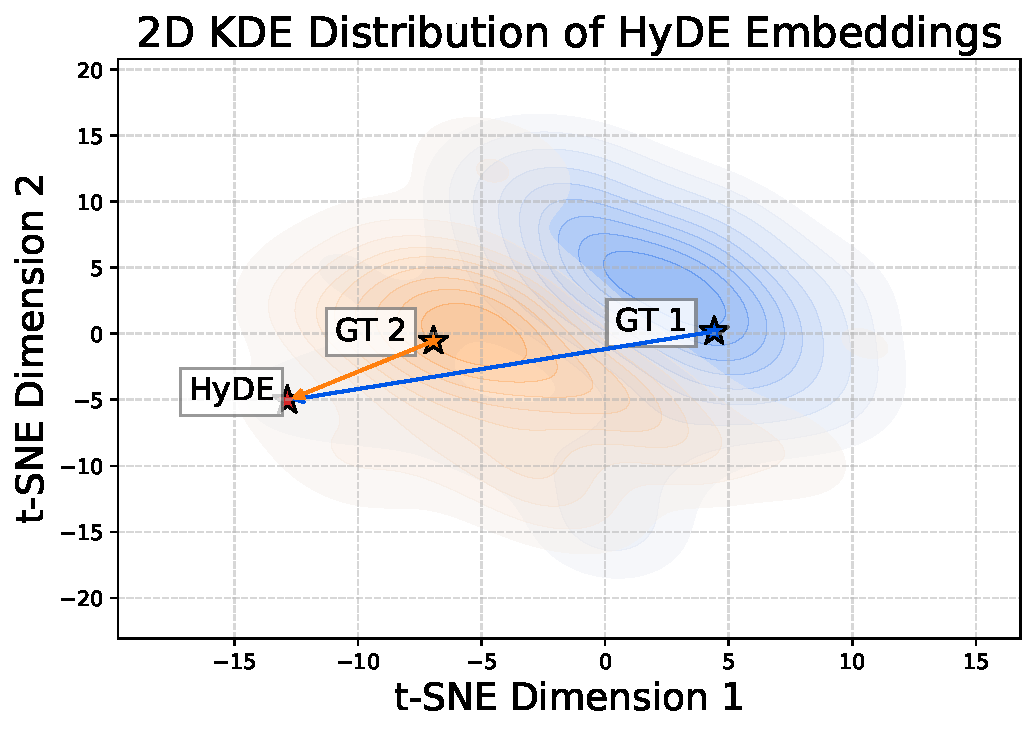
\includegraphics[width=1.0\linewidth]{figure/figure2_hyde_gt.pdf}
    \caption{HyDE-GT Comparison}
    \label{fig:hyde_gt}
  \end{subfigure}
  \hfill
  \begin{subfigure}[t]{0.32\textwidth}
    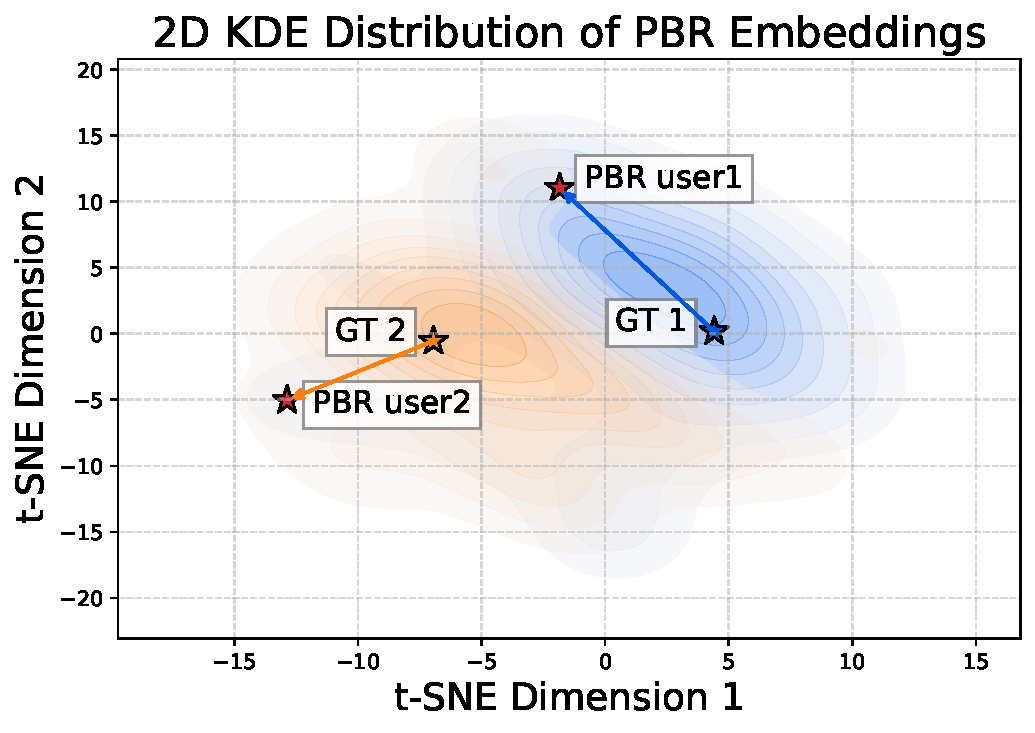
\includegraphics[width=1.0\linewidth]{figure/figure3_ours_gt.pdf}
    \caption{PBR-GT Comparison (Ours)}
    \label{fig:ours_gt}
  \end{subfigure}
  \caption{Visualization of retrieval distance of the query in the Figure~\ref{fig:intro} compared to ground truth (GT) under different methods: (a) vanilla query, (b) HyDE, and (c) our proposed PBR.}
  \label{fig:retrieval_gt_comparison}
  \vspace{-10pt}
\end{figure*}


To verify how information propagation within the P-Anchor module influences the alignment between queries and user-specific semantic space, we conduct a sensitivity analysis over two structural hyperparameters: the semantic threshold $\theta$ and the neighbor size $k_2$. The results are shown in Figure~\ref{fig:anchor_sensitivity}.

\textbf{Moderate propagation improves alignment.} When $\theta \in [0.65, 0.75]$ and $k_2 = 5$, both R@5 and N@5 reach consistent peaks across datasets, indicating that controlled expansion of semantic neighborhoods facilitates better anchoring and personalization.

\textbf{Over-propagation causes semantic drift.} As $\theta$ and $k_2$ continue to increase, performance either saturates or slightly declines (e.g., at $\theta=0.8$, $k_2=10$), suggesting that excessive propagation introduces noise and weakens the semantic specificity of the alignment.

\subsection{Visualization Case Study}

To verify the practical effectiveness of our proposed PBR framework, we conduct a retrieval visualization case study.
Figure~\ref{fig:retrieval_gt_comparison} visualizes the t-SNE distribution of user queries, ground truths (GT), and generated queries under different methods.
The results show that traditional expansion methods produce generic results misaligned with different users.
Measuring cosine similarity to user-specific ground truth, PBR achieves higher separation between users (0.31 vs. 0.27), outperforming HyDE (0.04 vs. –0.01) and the original query (0.05 vs. 0.10). This highlights PBR’s effectiveness in embedding user-personalized semantics.

\textbf{P-PRF enables semantically diverse and intent-aligned queries.}
% Figure~\ref{fig:retrieval_gt_comparison} visualizes the t-SNE distribution of user queries, ground truths (GT), and generated queries under different methods.
Compared to vanilla queries or HyDE-generated expansions, PBR-generated queries are semantically closer to ground truth responses in both user clusters.
The trajectory of PBR vectors more accurately captures user-relevant preferences, confirming its effectiveness in generating expressive and personalized query variants.

\textbf{Improved alignment leads to more successful retrieval.}
Unlike HyDE, which generates a generic QE of all users, PBR yields multiple expansions (e.g., PBR user1 and PBR user2) that better cover the user-specific semantic space.
This personalized QE allows the retriever to more precisely locate relevant results near each GT, reducing retrieval distance and improving semantic alignment.


\FloatBarrier